\subsubsubsection{Incoming}
The Incoming application is responsible of receiving messages from other
middleware nodes and to dispatch these messages to the appropriate middleware
application.
However, before dispatching this component process the message by applying some
checks: in fact, a message may be directed to another node or it might have to
be withheld if a snapshot is occurring.

Therefore, we decided to take advantage of Elixir's
\href{https://hexdocs.pm/gen_stage/GenStage.html}{GenStage} behaviour and
structure the modules of this component as a pipeline through which the
message is processed:

\begin{figure}[H]
  \centering
  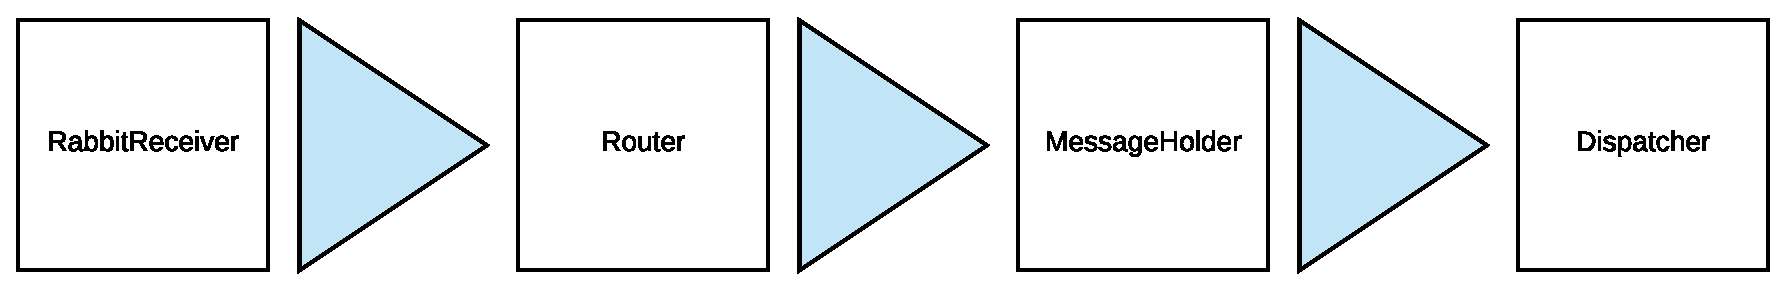
\includegraphics[width=\columnwidth]{images/solution/mw/inc/architect.eps}
  \caption{Incoming pipeline}
  \label{fig:mw-incoming}
\end{figure}

\begin{itemize}
  \item A RabbitReceiver is a process which receives messages from a single
    adjacent middleware node (or ``neighbor'') using RabbitMQ
  \item A Router compares the recipient field of the message with the
    identifier of the current node. If it is different, then it forwards the
    message to the next node along the path to the recipient
  \item A MessageHolder prevents messages to reach the dispatching point if a
    snapshot is happening. Then, when the snapshot ends, the messages will be
    forwarded again towards the Dispatcher
  \item A Dispatcher dispatches messages to a given application of the middleware
\end{itemize}

\begin{figure}[H]
  \centering
  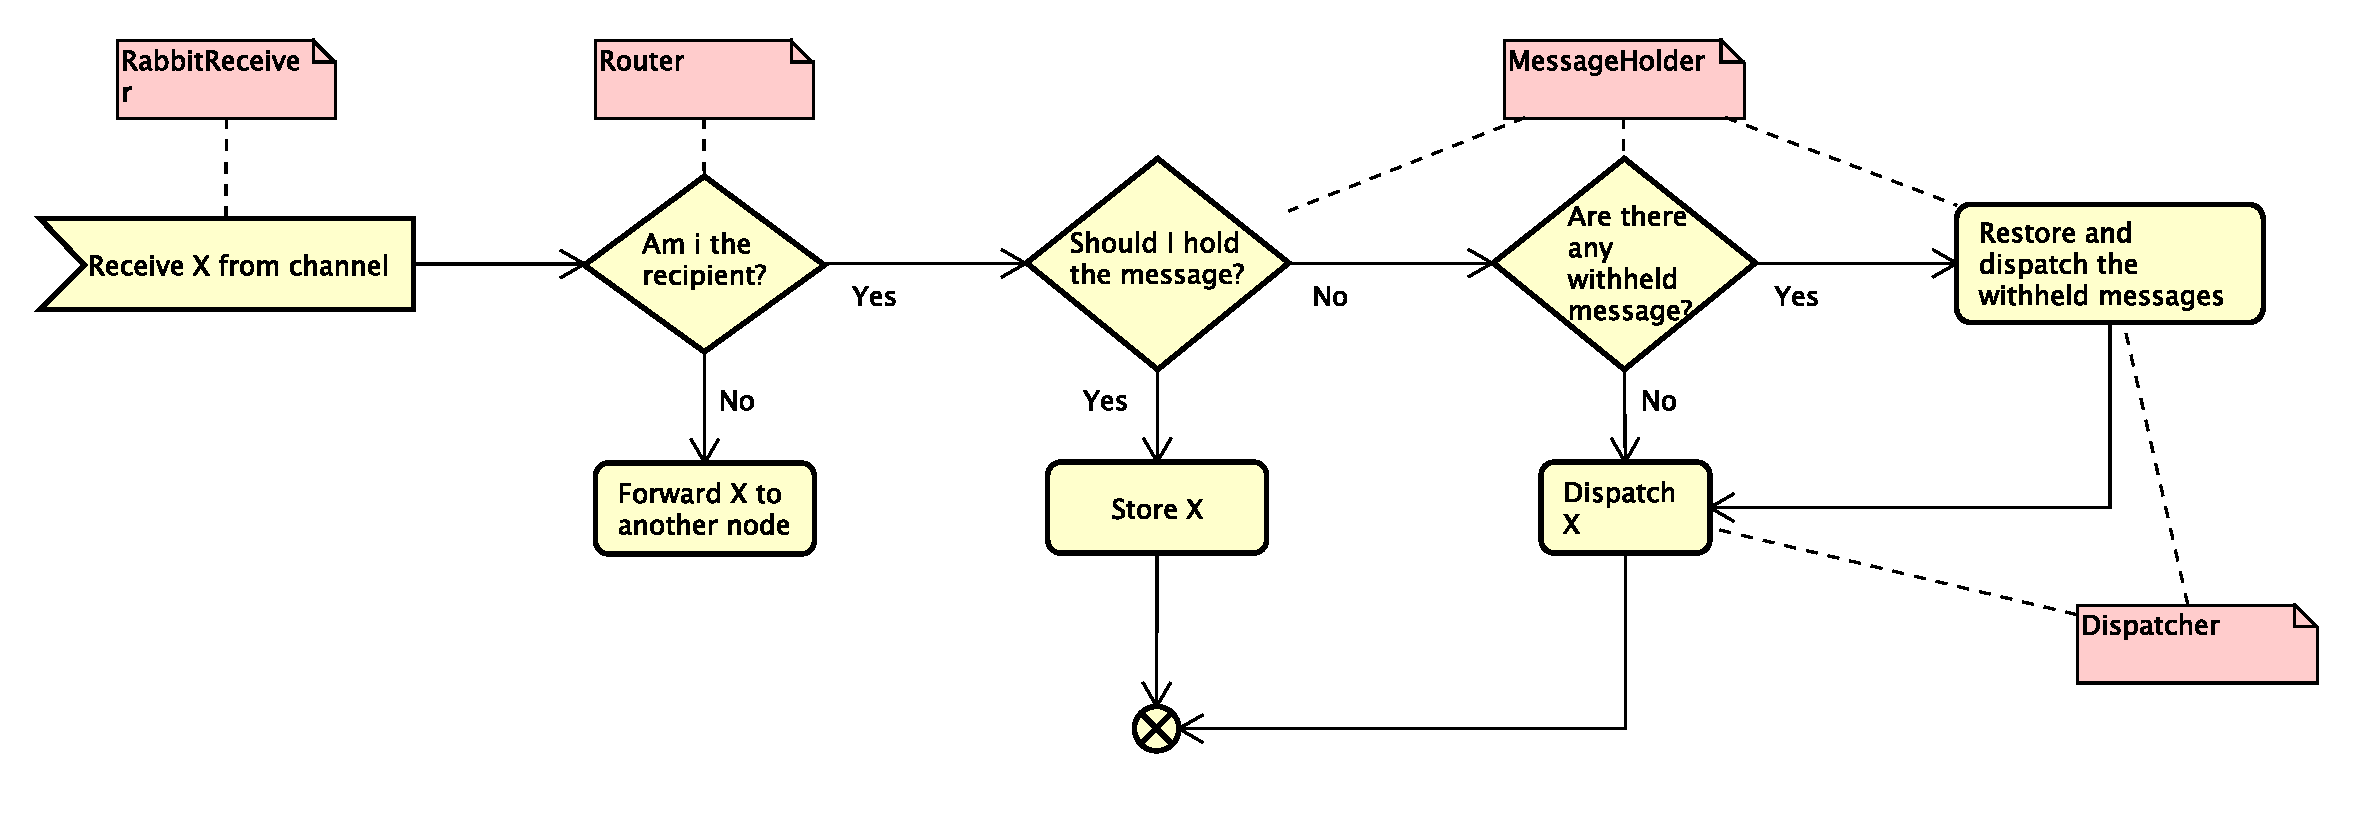
\includegraphics[width=\columnwidth]{images/solution/mw/inc/activity.eps}
  \caption{Activity diagram for Incoming pipeline}
  \label{fig:mw-incoming-activity}
\end{figure}

Thanks to the flexibility of GenStage, we can compose our pipelines by adding
an arbitrary number of elements at each stage of the pipeline. For instance,
there is one RabbitReceiver for each middleware neighbor plus one for loopback
communication: in this case, we just have to spawn as many RabbitReceivers as
needed and then make the Router subscribe to the events generated by them
(that is, the incoming messages).
